\documentclass[border=10pt]{standalone}

\usepackage{tikz}
\usepackage{tikzsymbols}
\usetikzlibrary{calc,patterns,shapes.geometric}

\def\centerarc[#1](#2)(#3:#4:#5){\draw[#1] ($(#2)+({#5*cos(#3)},{#5*sin(#3)})$) arc (#3:#4:#5);}

\begin{document}
	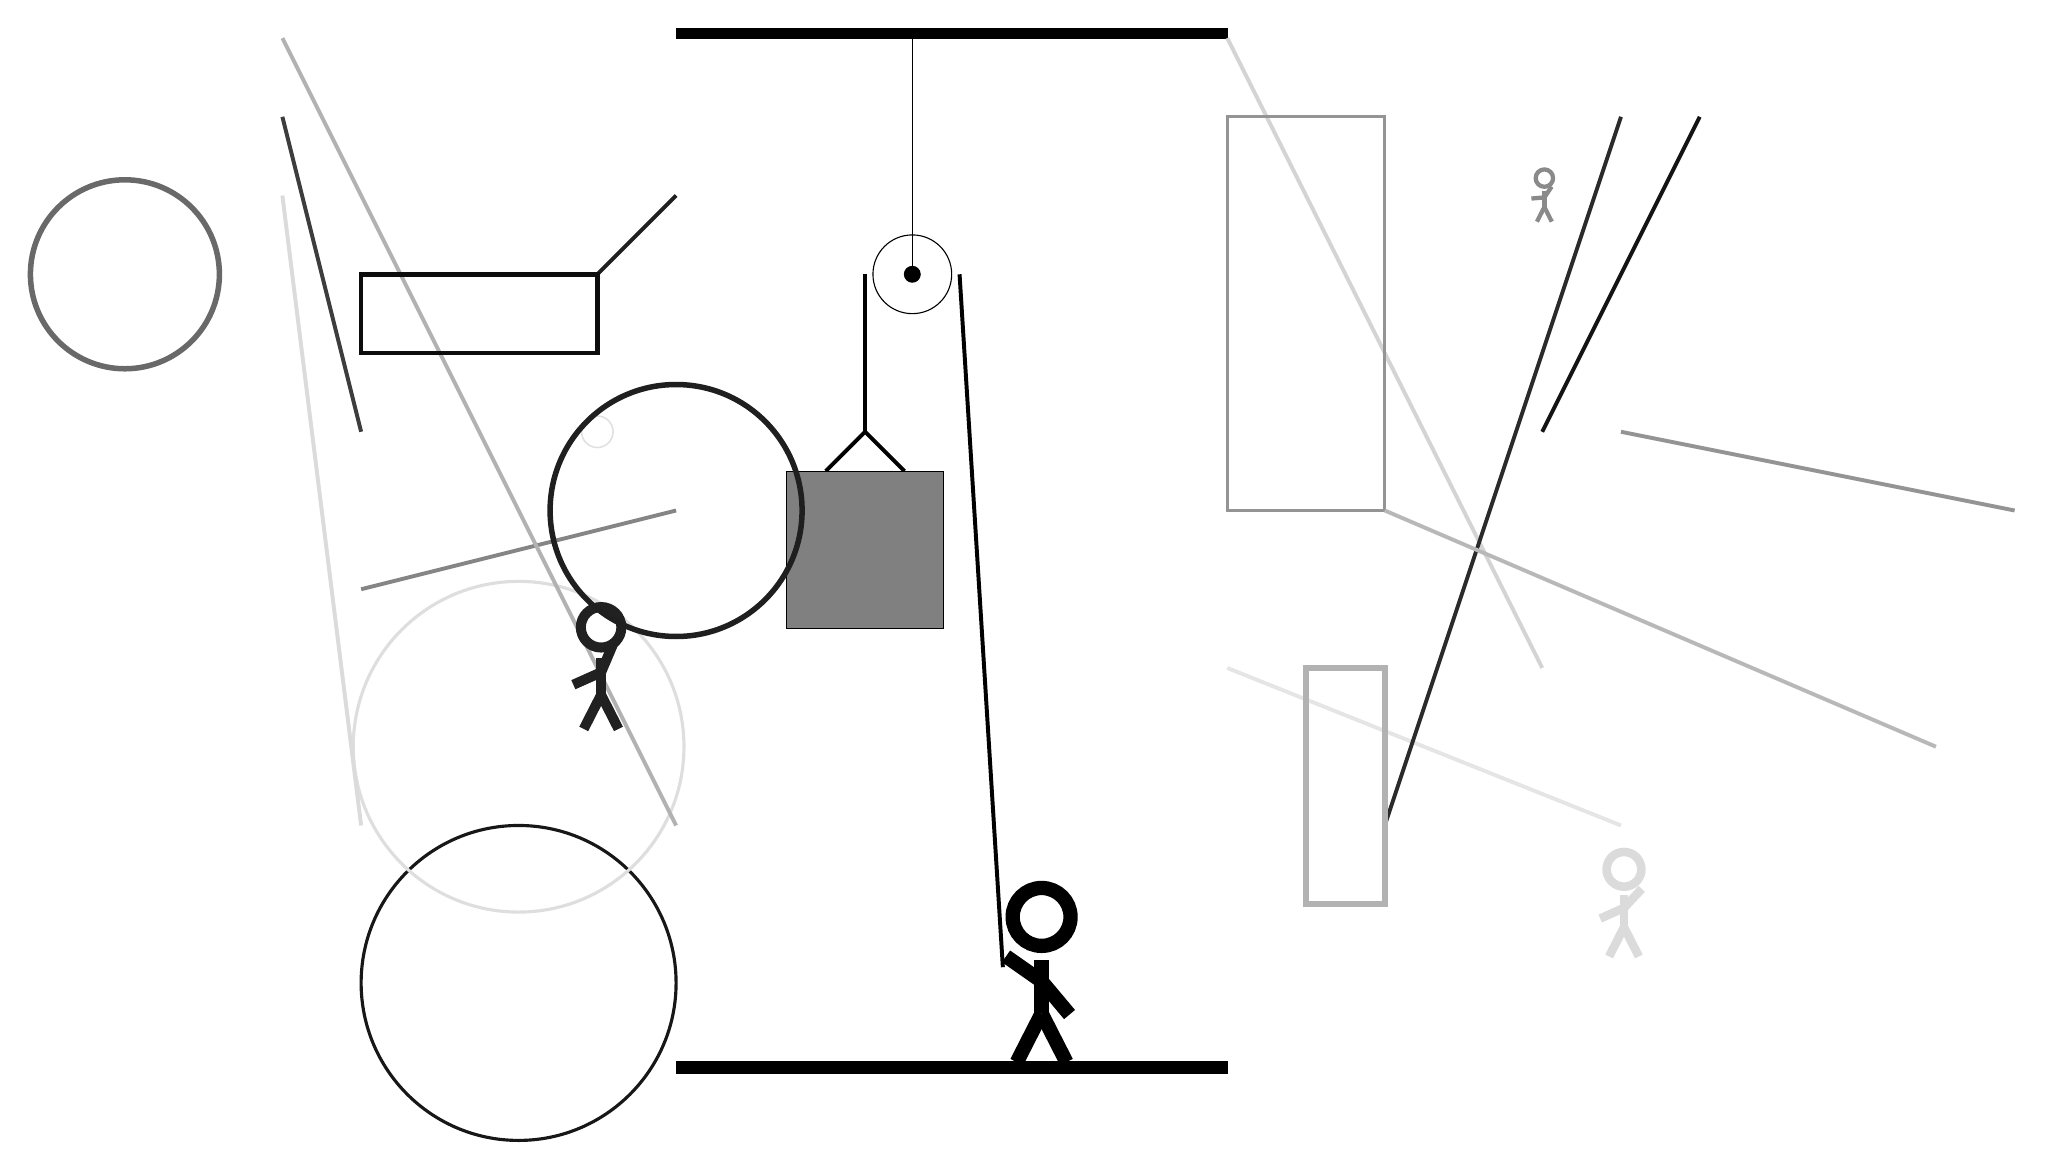
\begin{tikzpicture}
		%%%%% START %%%%%
		
		\draw[fill=black] (-2, 10) rectangle (5, 10.125);
		
		\draw (1, 7) circle (0.5);
		\draw[fill=black] (1, 7) circle (0.1);
		\draw (1, 10) -- (1, 7);
		
		\draw[line width=0.5mm] (-0.1, 4.5) -- (0.4, 5.0) -- (0.9, 4.5);
		\draw[fill=black!50] (-0.6, 4.5) rectangle (1.4, 2.5);
		
		\draw[line width=0.5mm, color=black!17](5, 10) -- (9, 2);
		
		\draw[line width=0.5mm, color=black!10](10, 0) -- (5, 2);
		\node[line width=0.7mm, color=black!14] at (10, -1) {\Strichmaxerl[6][24][47]};
		\draw[line width=0.5mm, color=black!76](-7, 9) -- (-6, 5);
		\draw[line width=0.4mm, color=black!42] (7, 4) rectangle (5, 9);
		\node[line width=0.6mm, color=black!46] at (9, 8) {\Strichmaxerl[3][5][56]};
		\draw[line width=0.5mm, color=black!48](-2, 4) -- (-6, 3);
		
		\draw[line width=0.5mm, color=black!88](-3, 7) -- (-2, 8);
		\draw[line width=0.5mm, color=black!42](10, 5) -- (15, 4);
		\draw [line width=0.4mm, color=black!91](-4, -2) circle (2.0);
		
		\draw[line width=0.5mm, color=black!92](9, 5) -- (11, 9);
		\draw [line width=0.4mm, color=black!13](-4, 1) circle (2.1);
		\draw [line width=0.2mm, color=black!12](-3, 5) circle (0.2);
		\draw[line width=0.5mm, color=black!83](7, 0) -- (10, 9);
		\draw[line width=0.5mm, color=black!14](-7, 8) -- (-6, 0);
		\draw[line width=0.5mm, color=black!30](-7, 10) -- (-2, 0);
		
		\draw[line width=0.6mm, color=black!95] (-3, 6) rectangle (-6, 7);
		\draw[line width=0.5mm, color=black!28](7, 4) -- (14, 1);
		\draw[line width=0.7mm, color=black!30] (6, 2) rectangle (7, -1);
		
		\draw [line width=0.7mm, color=black!59](-9, 7) circle (1.2);
		\node[line width=0.4mm, color=black!87] at (-3, 2) {\Strichmaxerl[7][24][67]};
		\draw [line width=0.7mm, color=black!88](-2, 4) circle (1.6);
		
		\draw[line width=0.5mm] (0.4, 7) -- (0.4, 5.0);
		\centerarc[line width=0.5mm](1, 7)(0:180:0.6);
		\draw[line width=0.5mm](1.6, 7) -- (2.15, -1.8);
		
		\node at (2.6, -1.9) {\Strichmaxerl[10][-35][-50]};
		
		\draw[fill=black] (-2, -3) rectangle (5, -3.15);
		
		%%%%% END %%%%%
	\end{tikzpicture}
\end{document}